\documentclass[12pt]{letter}
\usepackage{amsmath,amsfonts,amsthm,amstext,amssymb,graphicx, multicol,fancyhdr,lastpage,fullpage,framed,fancybox,enumerate,tikz,color,mathrsfs, polynom, pifont, stmaryrd}
\usepackage[margin=0.6in,headsep=3pt, headheight=15pt]{geometry}

% ----------------------------------------------------------
% Custom Definitions, Commands, Environments, etc.

% Sets of numbers
\def\R{\mathbb{R}} % The reals
\def\N{\mathbb{N}} % The naturals
\def\Z{\mathbb{Z}} % The integers
\def\Q{\mathbb{Q}} % The rationals

% Blank space
\newcommand{\blank}[1]{\underline{\hspace{#1}}} % Blank space

% Change font colors
\newcommand{\cyan}[1]{{\color{cyan}{#1}}} % Changes font to cyan
\newcommand{\red}[1]{{\color{red}{#1}}} % Changes font to red
\newcommand{\magenta}[1]{{\color{magenta}{#1}}} % Changes font to magenta
\newcommand{\orange}[1]{{\color{orange}{#1}}} % Changes font to orange
\newcommand{\yellow}[1]{{\color{yellow}{#1}}} % Changes font to yellow
\newcommand{\violet}[1]{{\color{violet}{#1}}} % Changes font to violet
\newcommand{\green}[1]{{\color{green}{#1}}} % Changes font to green
\newcommand{\blue}[1]{{\color{blue}{#1}}} % Changes font to blue
\newcommand{\white}[1]{{\color{white}{#1}}} % Changes font to white

% Fitted inclusion symbols
\newcommand{\fp}[1]{\left({#1}\right)} % Fitted parentheses around content
\newcommand{\fb}[1]{\left[{#1}\right]} % Fitted brackets
\newcommand{\lhoi}[1]{\left({#1}\right]} % Left half-open interval
\newcommand{\rhoi}[1]{\left[{#1}\right)} % Right half-open interval
\newcommand{\set}[1]{\left\{{#1}\right\}} % Fitted braces (useful for sets)
\newcommand{\av}[1]{\left|{#1}\right|} % Fitted absolute value bars
\newcommand{\step}[1]{\left\llbracket {#1} \right\rrbracket}

% Augmented Matrix Environment
\newenvironment{amatrix}[1]{%
	\left[\begin{array}{@{}*{#1}{c}|c@{}}
	}{%
	\end{array}\right]
}

% Miscellaneous
\def\then{\Rightarrow}
\def\to{\rightarrow}
\def\d{^{\circ}}
\newcommand{\?}{\stackrel{?}{=}}
\newcommand{\cmark}{\text{ \ding{51}}}
\newcommand{\xmark}{\text{ \ding{55}}}



% Coordinate Plane (Four-Quadrant)
\def\coordplane {
	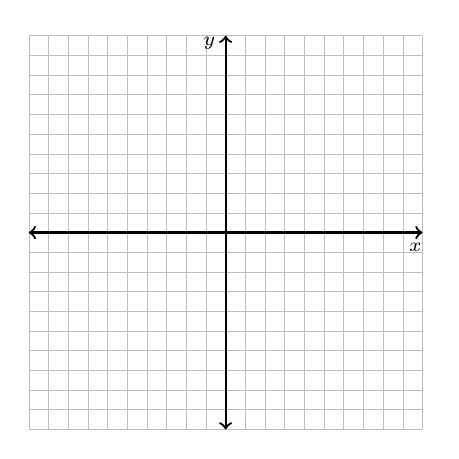
\begin{tikzpicture}        \draw[step=0.25cm,black,very thin,opacity=0.25] (-2.5cm, -2.5cm) grid (2.5cm, 2.5cm);
	\draw[<->,thick,black] (-2.5cm, 0) -- (2.5cm, 0) node[anchor=north west,pos=0.94,font=\scriptsize]{$x$};
	\draw[<->,thick,black] (0,-2.5cm) -- (0, 2.5cm) node[anchor=south east,font=\scriptsize,pos=0.94]{$y$};
	\end{tikzpicture}
}

% Coordinate Plane (One-Quadrant)
\def\onequad {
	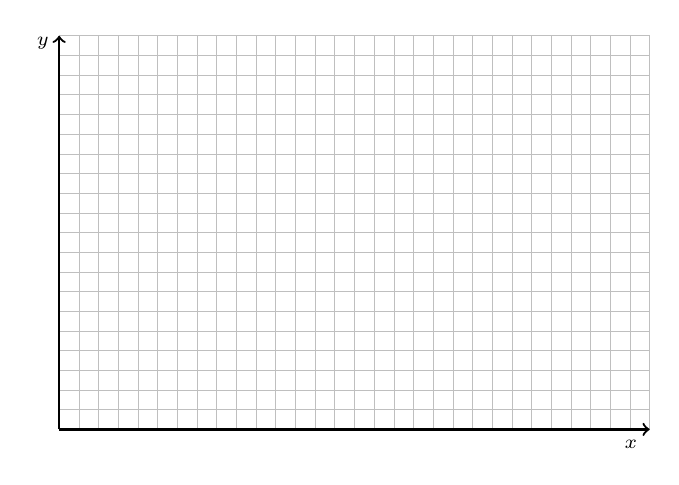
\begin{tikzpicture}
	\draw[step=0.25cm, black, very thin, opacity=0.25] (0,0) grid (7.5cm,5cm);
	\draw[->, thick, black] (0,0) -- (7.5cm, 0) node[anchor=north west,font=\scriptsize,pos=0.94]{$x$};
	\draw[->, black, thick] (0,0) -- (0,5cm) node[anchor=south east,font=\scriptsize,pos=0.94]{$y$};
	\end{tikzpicture}
}

% Counters
\newcounter{exercise}

% Exercise environment (auto-numbered)
\newenvironment{exercise}[1][]{\begin{framed}\refstepcounter{exercise}\textbf{Exercise~\theexercise:} #1}{\end{framed}}

% Book exercise environment
\newenvironment{bex}[2] {
	\begin{framed}
		\textbf{Book Exercise {#1}:} #2
	\end{framed}	
}
% ----------------------------------------------------------

% ----------------------------------------------------------
% Header and Footer Information
% \pagestyle{fancy}
% \fancyhf{}
% \renewcommand{\headrulewidth}{0pt}
% \rhead{Name: \blank{2in}}
% \lhead{@}
% \rfoot{Page \thepage \, of \,\pageref{LastPage}}
% ----------------------------------------------------------
\author{Jacob Ayers}

\begin{document}

\textbf{Midterm 1 KEY \\ MAT 130}


\begin{exercise}
	Evaluate $x^2 + 7x -3$ when $x = -3$. \begin{enumerate}[A.]
		\red{\item $-15$}
		\item $27$
		\item $0$
		\item $-33$
	\end{enumerate}
\end{exercise}

% My answer here
\vspace{-32pt} \begin{flalign*}
(-3)^2 + 7(-3) - 3 &= 9 - 21 - 3 & \\
&= -15
\end{flalign*}

\vfill % \newpage

\begin{exercise}
	Simplify the expression $\fp{4a}^3\fp{5a^2}$. \begin{enumerate}[A.]
		\item $320a^6$
		\item $20a^5$
		\red{\item $320a^5$}
		\item $20a^6$
	\end{enumerate}
\end{exercise}

% My answer here
\vspace{-32pt} \begin{flalign*}
\fp{4a}^3\fp{5a^2} &= 4^3 \cdot a^3 \cdot 5 \cdot a^2 & \\
&= 64 \cdot 5 \cdot a^5 & \\
&= 320a^5
\end{flalign*}

\vfill % \newpage

\begin{exercise}
	Find the product: $\fp{2x - 3}^2$. \begin{enumerate}[A.]
		\red{\item $4x^2 - 12x + 9$}
		\item $4x^2 + 9$
		\item $4x^2 + 12x + 9$
		\item $2x^2 - 6x + 9$
	\end{enumerate}
\end{exercise}

% My answer here
\vspace{-32pt} \begin{flalign*}
\fp{2x - 3}^2 = (2x - 3)(2x - 3) & \\
&= 4x^2 - 6x - 6x + 9 & \\
&= 4x^2 - 12x + 9
\end{flalign*}

\vfill \newpage

\begin{exercise}
	Factor completely: $27x^3 - 8$. \begin{enumerate}[A.]
		\item $(3x + 2)(3x-2)$
		\item $(3x - 2)^3$
		\item $(3x + 2)\fp{9x^2 - 6x + 4}$
		\red{\item $\fp{3x - 2}\fp{9x^2 + 6x + 4}$}
	\end{enumerate}
\end{exercise}

% My answer here
$u = x$ \\
$v = 3$

To factor the difference of two cubes: $(u - v)\fp{u^2 + uv + v^2}$

Factored result: $(x - 3)\fp{x^2 + 3x + 9}$


\vfill % \newpage

\begin{exercise}
	Find the domain of the expression: $\sqrt{x - 8}$. \begin{enumerate}[A.]
		\item $[-8, \infty)$
		\red{\item $[8, \infty)$}
		\item $(-\infty, 8]$
		\item $(-\infty, -8]$
	\end{enumerate}
\end{exercise}

% My answer here
\vspace{-32pt} \begin{flalign*}
x - 8 &\geq 0 & \\
x &\geq 8
\end{flalign*}
As an interval: $[8, \infty)$

\vfill \newpage

\begin{exercise}
	Perform the operation and simplify: $\dfrac{x^2 - 7x + 12}{x^2 + 8x + 16} \cdot \dfrac{x + 4}{x^2 - 9}$ \begin{enumerate}[A.]
		\item $\dfrac{1}{(x+4)(x+3)}$
		\red{\item $\dfrac{x-4}{(x+4)(x+3)}$}
		\item $x - 4$
		\item $\dfrac{x+4}{(x-4)(x+3)}$
	\end{enumerate}
\end{exercise}

% My answer here
\vspace{-32pt} \begin{flalign*}
\dfrac{x^2 - 7x + 12}{x^2 + 8x + 16} \cdot \dfrac{x + 4}{x^2 - 9} &= \dfrac{(x - 4)(x - 3)}{(x + 4)(x + 4)} \cdot \dfrac{x + 4}{(x + 3)(x - 3)} & \\
&= \dfrac{x - 4}{(x + 4)(x + 3)}
\end{flalign*}

\vfill % \newpage

\begin{exercise}
	To the nearest hundredth, find the distance between $\fp{-3.5, 6.1}$ and $\fp{2.8, 9.9}$. \begin{enumerate}[A.]
		\item $8.41$
		\item $3.86$
		\red{\item $7.36$}
		\item $16.02$
	\end{enumerate}
\end{exercise}

% My answer here
\vspace{-32pt} \begin{flalign*}
D &= \sqrt{\fp{x_2 - x_1}^2 + \fp{y_2 - y_1}^2} & \\
&= \sqrt{\fp{2.8 - (-3.5)}^2 + \fp{9.9 - 6.1}^2} & \\
&= \sqrt{6.3^2 + 3.8^2} & \\
&= \sqrt{54.13} & \\
&\approx 7.36
\end{flalign*}

\vfill \newpage

\begin{exercise}
	Test the equation $y = \av{x} - 4$ for symmetry about both axes. \begin{enumerate}[A.]
		\item Symmetric about both the $x$-axis and the $y$-axis
		\item Symmetric about neither the $x$-axis nor the $y$-axis
		\item Symmetric about the $x$-axis
		\red{\item Symmetric about the $y$-axis}
	\end{enumerate}
\end{exercise}

% My answer here
Test for $x$-axis: Replace $y$ with $-y$ \\
$-y = |x| - 4 \then y = -|x| + 4$ \\
Not symmetric

Test for $y$-axis: Replace $x$ with $-x$ \\
$y = |-x| - 4 \then y = |x| - 4$ \\
Symmetric

Test for origin: Replace $y$ with $-y$ and $x$ with $-x$ \\
Not symmetric (replacing $y$ with $-y$ didn't work before and won't work now either)

\vfill % \newpage

\begin{exercise}
	Solve for $x$: $\dfrac{x}{4} - 5 = \dfrac{x}{5} + 6$. \begin{enumerate}[A.]
		\item $240$
		\item $180$
		\item $200$
		\red{\item $220$}
	\end{enumerate}
\end{exercise}

% My answer here
\vspace{-32pt} \begin{flalign*}
20\fp{\dfrac{x}{4} - 5} &= 20\fp{\dfrac{x}{5} + 6} & \\
5x - 100 &= 4x + 120 & \\
x &= 220
\end{flalign*}

\vfill \newpage

\begin{exercise}
	Which of the following is the $x$-intercept of the equation $3x + 8y = 48$? \begin{enumerate}[A.]
		\red{\item $(16, 0)$}
		\item $(0, 16)$
		\item $(6, 0)$
		\item $(0, 6)$
	\end{enumerate}
\end{exercise}

% My answer here
Setting $y = 0$: \\
$3x + 8(0) = 48 \then 3x = 48 \then x = 16$

$x$-intercept is $(16, 0)$

\vfill % \newpage

\begin{exercise}
	Solve for $r$: $V = \pi r^2 h$ \begin{enumerate}[A.]
		\item $r = \fp{\dfrac{V}{\pi h}}^2$
		\red{\item $r = \sqrt{\dfrac{V}{\pi h}}$}
		\item $r = \fp{\pi h V}^2$
		\item $r = \sqrt{\pi h V}$
	\end{enumerate}
\end{exercise}

% My answer here
\vspace{-25pt} \begin{flalign*}
V &= \pi r^2 h & \\
r^2 &= \dfrac{V}{\pi h} & \\
r &= \sqrt{\dfrac{V}{\pi h}}
\end{flalign*}

\vfill \newpage

\begin{exercise}
	Solve for $x$: $-2x^2 - 5x + 27 = 0$ \begin{enumerate}[A.]
		\item $x = \dfrac{-5 \pm \sqrt{241}}{2}$
		\item $x = \dfrac{5 \pm \sqrt{241}}{2}$
		\item $x = \dfrac{5 \pm \sqrt{241}}{4}$
		\red{\item $x = \dfrac{-5 \pm \sqrt{241}}{4}$}
	\end{enumerate}
\end{exercise}

% My answer here
\vspace{-32pt} \begin{flalign*}
x &= \dfrac{-b \pm \sqrt{b^2 - 4ac}}{2a} & \\
&= \dfrac{-(-5) \pm \sqrt{(-5)^2 - 4(-2)(27)}}{2(-2)} & \\
&= \dfrac{5 \pm \sqrt{25 + 216}}{-4} & \\
&= \dfrac{-5 \pm \sqrt{241}}{4}
\end{flalign*}

\vfill % \newpage

\begin{exercise}
	Write the quotient in standard form: $\dfrac{4 - 3i}{2 + 5i}$ \begin{enumerate}[A.]
		\item $\dfrac{23}{21} + \dfrac{26}{21}i$
		\item $\dfrac13 + \dfrac{26}{21}i$
		\red{\item $-\dfrac{7}{29}-\dfrac{26}{29}i$}
		\item $\dfrac{23}{29} - \dfrac{26}{29}i$
	\end{enumerate}
\end{exercise}

% My answer here
\vspace{-32pt} \begin{flalign*}
\dfrac{(4-3i)}{(2+5i)}\cdot \dfrac{(2 - 5i)}{(2 - 5i)} &= \dfrac{8 - 20i - 6i + 15i^2}{4 - 10i + 10i - 25i^2} & \\
&= \dfrac{-7 - 26i}{29} & \\
&= -\dfrac{7}{29} - \dfrac{26}{29}i
\end{flalign*}

\vfill \newpage

\begin{exercise}
	Which of the following is NOT a solution to the equation $x^3 - 7x^2 + 4x - 28 = 0$? \begin{enumerate}[A.]
		\item $-2i$
		\item $2i$
		\red{\item $-7$}
		\item $7$
	\end{enumerate}
\end{exercise}

% My answer here
This can be solved using factoring by grouping. \begin{flalign*}
x^3 - 7x^2 + 4x - 28 &= 0 & \\
x^2\fp{x - 7} + 4\fp{x - 7} &= 0 & \\
\fp{x^2 + 4}\fp{x - 7} &= 0 & \\
x^2 + 4 &= 0 \then x = \pm 2i & \\
x - 7 &= 0 \then x = 7
\end{flalign*}
The only number listed that isn't a solution is $-7$.

\vfill % \newpage

\begin{exercise}
	Solve for $x$: $-3\fp{x - 5} \leq 4x - 13$ \begin{enumerate}[A.]
		\red{\item $x \geq 4$}
		\item $x \leq 4$
		\item $x \geq -4$
		\item $x \leq -4$
	\end{enumerate}
\end{exercise}

% My answer here
\vspace{-32pt} \begin{flalign*}
-3(x-5) &\leq 4x - 13 & \\
-3x + 15 &\leq 4x - 13 & \\
-7x + 15 &\leq -13 & \\
-7x &\leq -28 & \\
x &\geq 4
\end{flalign*}

\vfill \newpage

\begin{exercise}
	Which of the following is the solution to the inequality $x^2 + 4x - 45 < 0$? \begin{enumerate}[A.]
		\item $[-9, 5]$
		\red{\item $(-9, 5)$}
		\item $(-\infty, -9] \cup [5, \infty)$
		\item $(-\infty, -9) \cup (5, \infty)$
	\end{enumerate}
\end{exercise}

% My answer here
First, find the zeros of the polynomial: \begin{flalign*}
x^2 + 4x - 45 &= 0 & \\
(x + 9)(x - 5) &= 0 & \\
x &= \set{-9, 5}
\end{flalign*}
This divides the real numbers into three intervals: $(-\infty, -9), (-9, 5), (5, \infty)$. \\
Pick one number from each to test.

$(-\infty, -9)$: Test $-10$; result: $15$ which is larger than zero. This rules out answer choices $C$ and $D$.

$(-9, 5)$: Test $0$; result: $-45$ which is less than zero. This interval works.

Correct answer: $(-9, 5)$

\vfill % \newpage

\begin{exercise}
	Calculate the slope between $(-2, 8)$ and $(5, 20)$. \begin{enumerate}[A.]
		\item $\dfrac{28}{3}$
		\item $\dfrac{7}{12}$
		\item $\dfrac{3}{28}$
		\red{\item $\dfrac{12}{7}$}
	\end{enumerate}
\end{exercise}

% My answer here
\vspace{-32pt} \begin{flalign*}
m &= \dfrac{y_2 - y_1}{x_2 - x_1} & \\
&= \dfrac{20 - 8}{5 - (-2)} & \\
&= \dfrac{12}{7}
\end{flalign*}

\vfill \newpage

\begin{exercise}
	Find the slope-intercept form of the equation of a line passing through $(2, 4)$ and parallel to $y = 3x - 4$. \begin{enumerate}[A.]
		\red{\item $y = 3x - 2$}
		\item $y - 4 = 3(x - 2)$
		\item $y - 2 = 3(x - 4)$
		\item $y = 3x - 10$
	\end{enumerate}
\end{exercise}

% My answer here
Options B and C aren't written in slope-intercept form; they can be ruled out.

We need a line parallel to $y = 3x - 4$; parallel lines have the same slope, so our new line will have a slope of $3$. We also need the line to pass through $(2, 4)$. Substituting $x_1 = 2$ and $y_1 = 4$ into the point-slope formula: \begin{flalign*}
y - 4 &= 3(x - 2) & \\
y - 4 &= 3x - 6 & \\
y &= 3x - 2
\end{flalign*}

\vfill % \newpage

\begin{exercise}
	Consider the function $f$ given by $f(x) = x^{2/3}$. Evaluate $f(64)$. \begin{enumerate}[A.]
		\item $\dfrac{128}{3}$
		\item $64$
		\red{\item $16$}
		\item $512$
	\end{enumerate}
\end{exercise}

% My answer here
\vspace{-32pt} \begin{flalign*}
64^{2/3} &= \fp{\sqrt[3]{64}}^2 & \\
&= 4^2 & \\
&= 16
\end{flalign*}

\vfill \newpage

\begin{exercise}
	Find the zeros of the function $f(x) = 5x^2 + 4x + 1$. \begin{enumerate}[A.]
		\item $\set{-\dfrac15, 1}$
		\red{\item $\set{-1, \dfrac15}$}
		\item $\set{-1, -\dfrac15}$
		\item $\set{\dfrac15, 1}$
	\end{enumerate}
\end{exercise}

% My answer here
The polynomial can be factored. \begin{flalign*}
5x^2 + 4x + 1 &= 0 & \\
(5x - 1)(x + 1) &= 0 & \\
5x - 1 &= 0 \then x = \dfrac15 & \\
x + 1 &= 0 \then x = -1
\end{flalign*}

\vfill % \newpage

\begin{exercise}
	Which of the following is NOT a relative extremum of the function $g(x) = x^4 - 3x^2 + 2x + 4$? \begin{enumerate}[A.]
		\item $(1, 4)$
		\item $(0.37, 4.85)$
		\item $(-1.37, -0.85)$
		\red{\item $(-2.38, 5.16)$}
	\end{enumerate}
\end{exercise}

% My answer here
You'd need to use the Extremum tool in GeoGebra (provided on test) in order to answer this exercise.

\vfill \newpage

\begin{exercise}
	Identify the transformation of the parent function described by the function $h(x) = \sqrt{x + 5} + 2$. \begin{enumerate}[A.]
		\red{\item Parent function $f(x) = \sqrt{x}$, translated five units to the left and two units up.}
		\item Parent function $f(x) = \sqrt{x}$, translated five units to the right and two units up.
		\item Parent function $f(x) = \sqrt{x}$, translated five units to the left and two units down.
		\item Parent function $f(x) = \sqrt{x}$, translated five units to the right and two units down.
	\end{enumerate}
\end{exercise}

% My answer here
We have that $h = -5$ and $k = 2$. So the parent function is translated five units left and two units up.

\vfill % \newpage

\begin{exercise}
	Let $f(x) = 7x - 11$ and $g(x) = 4x + 19$. Find $f \circ g$. \begin{enumerate}[A.]
		\item $f \circ g = 28x - 25$
		\red{\item $f \circ g = 28x + 122$}
		\item $f \circ g = 11x + 8$
		\item $f \circ g = 28x^2 + 89x - 209$
	\end{enumerate}
\end{exercise}

% My answer here
\vspace{-32pt} \begin{flalign*}
f \circ g &= f\fb{g(x)} & \\
&= f\fp{4x + 19} & \\
&= 7(4x + 19) - 11 & \\
&= 28x + 133 - 11 & \\
&= 28x + 122
\end{flalign*}

\vfill \newpage

\begin{exercise}
	Based on the Horizontal Line Test, the function $f(x) = (x - 3)^2$ has an inverse. \begin{enumerate}[A.]
		\item True
		\red{\item False}
	\end{enumerate}
\end{exercise}

% My answer here
Here is the graph:

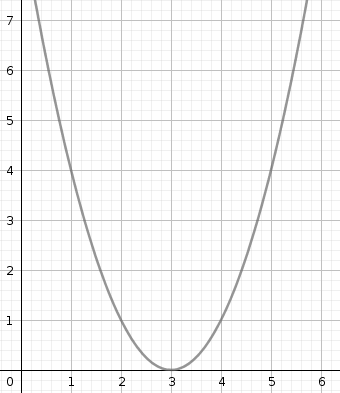
\includegraphics[width=2in]{24ans.png}

Clearly, we could find a horizontal line that would touch the graph twice. So the function does not have an inverse.

\vfill % \newpage

\begin{exercise}
	If $f(x) = \sqrt{x - 5}$, then find $f^{-1}(x)$. \begin{enumerate}[A.]
		\item $f^{-1}(x) = \sqrt{x - 5}$
		\item $f^{-1}(x) = x^2 - 5$
		\red{\item $f^{-1}(x) = x^2 + 5$}
		\item $f^{-1}(x) = \sqrt{x + 5}$
	\end{enumerate}
\end{exercise}

% My answer here
\vspace{-32pt} \begin{flalign*}
y &= \sqrt{x - 5} & \\
x &= \sqrt{y - 5} & \\
x^2 &= y - 5 & \\
x^2 + 5 &= y & \\
f^{-1}(x) &= x^2 + 5
\end{flalign*}

\vfill % \newpage


	
\end{document}